\documentclass[11pt]{article}

\usepackage{float}
\usepackage{hyperref}
\usepackage{fullpage}
\usepackage{verbatim}
\usepackage{moreverb}
\usepackage{graphicx}
\usepackage{parskip}

\usepackage{minted}
\let\verbatiminput=\verbatimtabinput
\def\verbatimtabsize{4\relax}

\begin{document}
\title{EECS 151/251A FPGA Lab\\
Lab 4: Serial I/O - UART}

\author{Prof. Elad Alon \\
TAs: Vighnesh Iyer, Bob Zhou \\
Department of Electrical Engineering and Computer Sciences\\
College of Engineering, University of California, Berkeley}
\date{}
\maketitle

\tableofcontents

\section{Before You Start This Lab}

Before you proceed with the contents of this lab, we suggest that you get acquainted with what a ready/valid handshake is. Read the document in \verb|labs_sp17/docs/Verilog/ready_valid_interface.pdf|. It may be helpful to draw out the timing diagrams for the ready/valid handshake to gain understanding. If you are having trouble, ask a TA. Please note that the serial line itself is not a ready/valid interface. Rather, it is the modules you will work with in this lab (\verb|UATransmit| and \verb|UAReceive|) that have the ready/valid handshake for interfacing with other modules on the FPGA.

In this lab you will implement a UART (Universal Asynchronous Receiver / Transmitter) device, otherwise known as a serial interface. Your working UART from this lab will be used in your project to talk to your workstation (desktop) over a serial line.

\textbf{This lab will be done individually, but the next 2 labs will be done with a partner.} If you have not found one yet, now is the time to do so. The deliverable for this lab will be used in your final project. Once you have a group of two, please email the TAs (bob.linchuan@berkeley.edu and vighnesh.iyer@berkeley.edu) with the names and Github ID's of both group members so that we can create your team project repositories. You can complete the lab without having your project repository yet; you'll only need it for the project.

\section{Lab Setup}
Run \verb|git pull| in the \verb|labs_sp17| folder to fetch the latest skeleton files. You will need to copy over your \verb|debouncer.v|, \verb|edge_detector.v|, and \verb|synchronizer.v| from Lab 3 to \verb|labs_sp17/lab4/src/|.

\section{Serial Device}
You are responsible only for implementing the \textbf{transmit} side of the UART for this lab. As you should have inferred from reading the ready/valid tutorial, the UART transmit and receive modules use a ready/valid interface to communicate with other modules on the FPGA.

Both the UART’s receive and transmit modules will have their own separate set of ready/valid interfaces connected appropriately to external modules.

\subsection{Framing}
On the \verb|ML505| board, the physical signaling aspects (such as voltage level) of the serial connection are taken care of by off-FPGA devices. From the FPGA's perspective, there are two signals, \verb|FPGA_SERIAL_RX| and \verb|FPGA_SERIAL_TX|, which correspond to the receive-side and transmit-side pins of the serial port. The FPGA's job is to correctly frame characters going back and forth across the serial connection. Figure 1 below shows a single character frame being transmitted and will be extremely useful in understanding the protocol.

\begin{figure}[H]
	\centerline{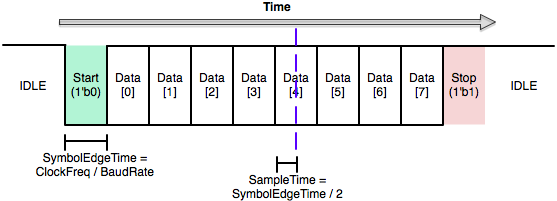
\includegraphics[width=6in]{images/uart_frame.png}}
	\caption{UART Frame Structure}
\end{figure}

In the idle state the serial line is held high. When the TX side is ready to send a character, it pulls the line low. This is called the start bit. Because UART is an asynchronous protocol, all timing within the frame is relative to when the start bit is first sent (or detected, on the receive side). 

The frame is divided up in to 10 uniformly sized bits: the start bit, 8 data bits, and then the stop bit. The width of a bit in cycles of the system clock is then naturally given by the system clock frequency divided by the baudrate. The baudrate is the number of bits sent per second; in this lab the baudrate will be 115200. Notice that both sides must agree on a baudrate for this scheme to be feasible.

\subsection{Transmitting}
Let us first think about sending a character using this scheme. Once we have a character that we want to send out, transmitting it is simply a matter of shifting each bit of the character, plus the start and stop bits, out of a shift register on to the serial line. 

Remember, the serial baudrate is much slower than the system clock, so we must wait $SymbolEdgeTime = \frac{ClockFreq}{BaudRate}$ cycles between changing the character we're putting on the serial line. After we have shifted all 10 bits out of the shift register, we are done unless we see another transmission immediately after.

\subsection{Receiving}
The receive side is a bit more complicated. Fortunately, we will provide the receiver module. Open \verb|lab4/src/uart_receiver.v| so you can see the explanation below implemented. 

Like the transmit side, the receive side of the serial device is essentially just a shift register, but this time we are shifting bits from the serial line into the shift register. However, care must be taken into determining when to shift bits in. If we attempt to sample the serial signal directly on the edge between two symbols, we are exceedingly likely to sample on the wrong side of the edge (or worse, when the signal is transitioning) and get the wrong value for that bit. The correct solution is to wait halfway into a cycle (until \verb|SampleTime| on the diagram) before reading a bit in to the shift register.

One other subtlety of the receive side is correctly implementing the ready/valid interface. Once we have received a full character over the serial port, we want to hold the valid signal high until the ready signal goes high, after which the valid signal will be driven low until we receive another character. 

This requires using an extra flip-flop (the \verb|has_byte| reg in \verb|uart_receiver.v|) that is set when the last character is shifted in to the shift register and cleared when the ready signal is asserted. This allows us to correctly implement the ready/valid handshake.

\subsection{Putting It All Together}
Although the receive side and transmit side of the UART you will be building are essentially orthogonal, we are packaging them into one UART module to keep things tidy. If you look at \verb|uart.v|, you will see that this module is mostly straightforward instantiations of \verb|uart_receiver| and \verb|uart_transmitter|, but there are also two \verb|iob| registers that the serial lines are fed through. What are these for? An \verb|iob| is simply a register that attempts to pack itself into a special block called an \verb|IOB|, which is used to drive and sense from the IO pins. Using an \verb|iob| helps ensure that you will have a nice, clean, well-behaved off-chip signal to use as an input or output to your serial modules.

The diagram below shows the entire setup:
\begin{figure}[H]
	\centerline{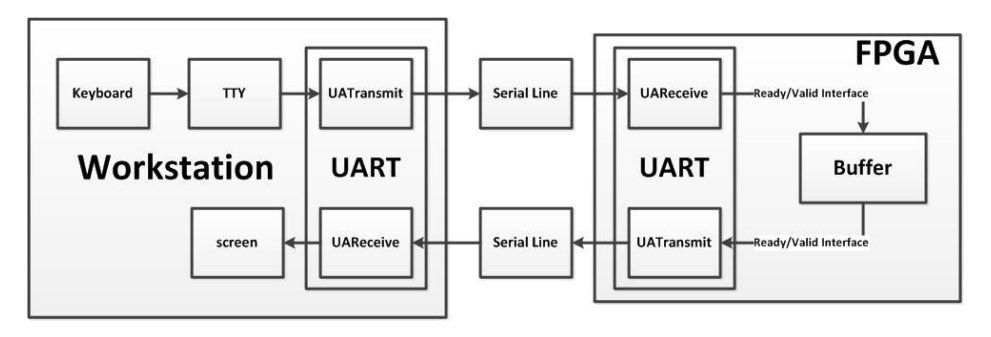
\includegraphics[width=6in]{images/high_level_diagram.png}}
	\caption{High Level Diagram}
\end{figure}

\subsection{Simulation}
We have provided a simple testbench, called \verb|uart_testbench| that will run some basic tests on two instantiations of the UART module with their RX and TX signals crossed so that they can talk to each other. There is also a \verb|.do| file that will run the test. You should note that this test bench reporting success is \textbf{not} by itself a good indication that your UART is working properly. The testbench does not attempt to test back to back UART transmissions so you will have to add that test in yourself. Due to the way x's are treated by Modelsim if many signals in your design are undefined the testbench may erroneously pass. Make sure to look at the waveform to see that everything appears to be working properly and that you adequately purge your simulation of high Z and undefined X signals. 

If the testbench prints out \verb|# <EOF>| it means that it timed out; this indicates that the testbench was stuck on a line, likely due to a condition that never became true. Inspect the waveform and match it up to the testbench code to see where it hangs and why. You shouldn't need to increase any of the timeouts in the \verb|.do| files.

\subsection{Echo}
Your UART will eventually be used to interact with your CPU from your workstation. Since you don't have a CPU yet, you need some other way to test that your UART works on the board.

We have provided this for you. The provided \verb|ml505top| contains a very simple finite state machine that does the following continuously:

\begin{itemize}
	\item Pulls a received character from the \verb|uart_receiver| using ready/valid
	\item If the received character is an ASCII letter (A-Z or a-z), its case is inverted (lower to upper case or upper or lower case)
	\item If the received character isn't an ASCII letter, it is unmodified
	\item The possibly modified character is sent to the \verb|uart_transmitter| using ready/valid to be sent over the serial line one bit at a time
\end{itemize}

Before programming your board, check with the provided \verb|echo_testbench.v| testbench that everything works as it should in simulation. This testbench is heavily commented to help you understand the communication between the 2 UARTs and the communication over the ready/valid interface. The file often refers to the UART on the workstation as the off-chip UART and the UART on the FPGA as the on-chip UART.

Once you have echo working in simulation, it is time to try it on the board. Synthesize your design and impact the board with it just like you have done in previous labs. You may see up to 3 warnings about \verb|rx_shift<0>| being unconnected or unused; these are expected and can be safely ignored.

Now, make sure the USB serial cable is plugged in between the ML505 board and your workstation and then run:

\begin{minted}{bash}
screen $SERIALTTY 115200
\end{minted}

This tells \verb|screen|, a highly versatile terminal emulator, to open up the serial device with a baud rate of 115200. When you type a character into the terminal, it is sent to the FPGA over the \verb|FPGA_SERIAL_RX| line, encoded in ASCII. The state machine in \verb|ml505top| may modify the character you sent it and will then push a new character over the \verb|FPGA_SERIAL_TX| line to your workstation. When \verb|screen| receives a character, it will display it in the terminal.

Now, if you have a properly working design, you should be able to tap a few characters into the terminal and have them echoed to you (with inverted case if you type letters). Make sure that if you type really fast that all characters still display properly. If you see some weird garbage symbols then the data is getting corrupted and something is likely wrong. If you see this happening very infrequently, don't just hope that it won't happen while the TA is doing the checkoff; take the time now to figure out what is wrong. UART bugs are a common source of headaches for groups during the first project checkpoint. 

To close \verb|screen|, type \verb|Ctrl-a| then \verb|Shift-k| and answer \verb|y| to the confirmation prompt. If you don't close screen properly, other students won't be able to access the serial port. Use \verb|screen -r| to re-attach an improperly closed screen session. Note that if \textbf{someone else} has forgotten to close \verb|screen| and thus locked the serial cable on your workstation, you will not be able to execute this command. Since we don’t have \verb|sudo| access on these machines, the only way to resolve this problem is to either find the offending user and have him kill his session, or reboot the computer.

\subsection{Checkoff}
Show your TA that you can successfully type characters on the keyboard and have them echoed back to display on your \verb|screen| session.

\end{document}